\documentclass{article}
\usepackage[UTF8]{ctex}
\usepackage[T1]{fontenc}
\usepackage[utf8]{inputenc}
\usepackage{float}
\usepackage{placeins}
\usepackage{latexsym}
\usepackage{amsmath}
\usepackage{amsthm}
\usepackage{listings}
\usepackage{xcolor}
\usepackage{ulem}
\usepackage{multicol}
\usepackage{geometry}
\usepackage{tikz}
\usetikzlibrary{positioning}
\usetikzlibrary[arrows, shapes, chains]

\lstset
{
    basicstyle = \ttfamily,
    keywordstyle = \bfseries\color{blue!70},
    commentstyle = \songti \upshape,
    escapeinside=``,
    breaklines = true,
    breakatwhitespace = true,
    breakautoindent = true,
    texcl = true,
    showstringspaces = false,
    basewidth = 0.5em,
    flexiblecolumns,
    columns = fixed,
    frame = {},
}
\lstdefinestyle{C}
{
    language = C,
}
\lstdefinestyle{Assembler}
{
    language = [X86masm]Assembler,
    alsolanguage = C,
}

\title{Homework 9}
\author{PB17000297 罗晏宸}
\date{November 10 2019}


\begin{document}

\maketitle

\section*{Exercise 1}
在Homework8 (1)中汇编代码上进行基本块划分,构建流图。

% \newgeometry{left = 10em, right = 10em}

\begin{multicols}{2}

\paragraph{解}
由以下汇编代码,划分基本块,给出如下流图:

\begin{lstlisting}[style = Assembler, lineskip = 0.2em]
.text
.globl  test
    .type   test, @function
test:
    pushl   %ebp
    movl    %esp, %ebp
    subl    $16, %esp
    movl    8(%ebp), %eax
    cmpl    12(%ebp), %eax
    jle     .L4
    cmpl    $0, 12(%ebp)
    je      .L4
    cmpl    $10, 12(%ebp)
    jle     .L4
    cmpl    $0, 8(%ebp)
    je      .L4
    cmpl    $20, 8(%ebp)
    jg      .L3
.L4:
    cmpl    $100, 8(%ebp)
    jg      .L3
    cmpl    $99, 12(%ebp)
    jle     .L2
    cmpl    $40, 8(%ebp)
    jg      .L2
    cmpl    $20, 12(%ebp)
    jle     .L3
    cmpl    $-10, 8(%ebp)
    jge     .L3
    jmp     .L2
.L3:
    movl    $100, -4(%ebp)
    jmp     .L5
.L2:
    movl    $60, -4(%ebp)
.L5:
    movl    -4(%ebp), %eax
    leave
    ret
        \end{lstlisting}
\end{multicols}

\begin{figure}[H]
    \centering
    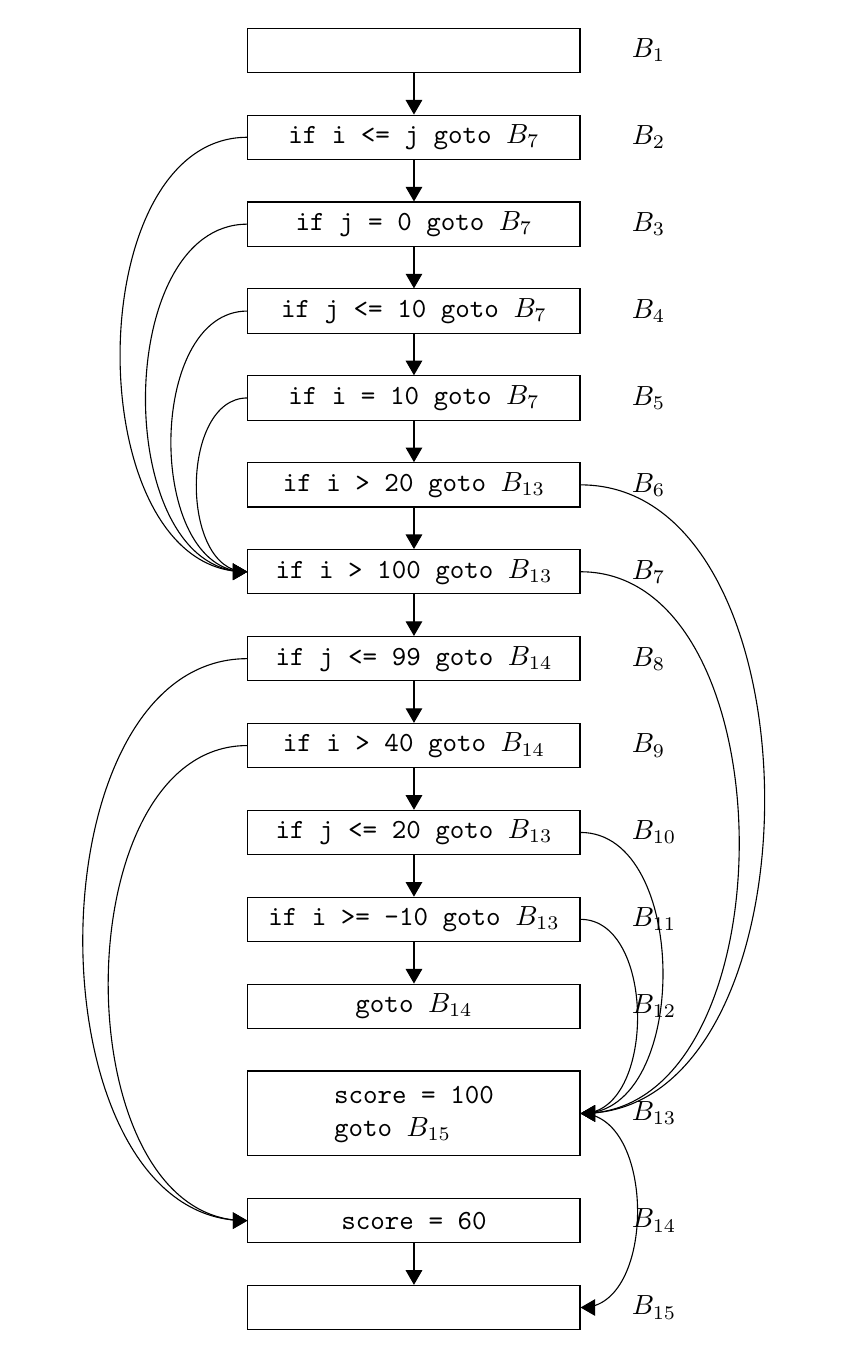
\begin{tikzpicture}[node distance = 1.5em]
        \tikzstyle{block} = [rectangle, draw=black, text ragged, minimum height = 1.6em, minimum width = 12em];
        \node [block]  (B1)  {};
        \node [block, below = of B1]  (B2)  {\texttt{if i <= j goto }$B_7$};
        \node [block, below = of B2]  (B3)  {\texttt{if j = 0 goto }$B_7$};
        \node [block, below = of B3]  (B4)  {\texttt{if j <= 10 goto }$B_7$};
        \node [block, below = of B4]  (B5)  {\texttt{if i = 10 goto }$B_7$};
        \node [block, below = of B5]  (B6)  {\texttt{if i > 20 goto }$B_{13}$};
        \node [block, below = of B6]  (B7)  {\texttt{if i > 100 goto }$B_{13}$};
        \node [block, below = of B7]  (B8)  {\texttt{if j <= 99 goto }$B_{14}$};
        \node [block, below = of B8]  (B9)  {\texttt{if i > 40 goto }$B_{14}$};
        \node [block, below = of B9]  (B10)  {\texttt{if j <= 20 goto }$B_{13}$};
        \node [block, below = of B10]  (B11)  {\texttt{if i >= -10 goto }$B_{13}$};
        \node [block, below = of B11]  (B12)  {\texttt{goto }$B_{14}$};
        \node [block, below = of B12]  (B13)
        {%
            \begin{tabular}{l}
                \texttt{score = 100} \\
                \texttt{goto }$B_{15}$
            \end{tabular}
        };
        \node [block, below = of B13]  (B14)  {\texttt{score = 60}};
        \node [block, below = of B14]  (B15)  {};
        \foreach \i in {1,..., 15}
            \node [right = of B\i] (A\i) {$B_{\i}$};
        \foreach \i/\j in {1/2, 2/3, 3/4, 4/5, 5/6, 6/7, 7/8, 8/9, 9/10, 10/11, 11/12, 14/15}
            \draw [-triangle 60] (B\i) to [] (B\j);

        \draw [-triangle 60] (B2) to [out = 180, in = 180] (B7);
        \draw [-triangle 60] (B3) to [out = 180, in = 180] (B7);
        \draw [-triangle 60] (B4) to [out = 180, in = 180] (B7);
        \draw [-triangle 60] (B5) to [out = 180, in = 180] (B7);
        \draw [-triangle 60] (B6) to [out = 0, in = 0] (B13);
        \draw [-triangle 60] (B7) to [out = 0, in = 0] (B13);
        \draw [-triangle 60] (B8) to [out = 180, in = 180] (B14);
        \draw [-triangle 60] (B9) to [out = 180, in = 180] (B14);
        \draw [-triangle 60] (B10) to [out = 0, in = 0] (B13);
        \draw [-triangle 60] (B11) to [out = 0, in = 0] (B13);
        \draw [-triangle 60] (B13) to [out = 0, in = 0] (B15);
    \end{tikzpicture}
    \caption{Homework8 (1)代码对应流图}
\end{figure}


% \restoregeometry
\section*{Exercise 2}
给出Homework1 (2)中C程序相应的三地址中间代码,并构建流图。

\paragraph{解}
由以下C语言代码

\begin{lstlisting}[style = C]
int main()
{
    int i, j = 0;
    for(i = 0; i < 10; i++)
    {
        switch(i)
        {
            case 0: case 2: break;
            case 3: case 5: continue;
            default: j = i;
        }
        L: j += i * 2;
    }
}
\end{lstlisting}

\end{document}

